\documentclass{llncs}


\usepackage{hyperref}
\usepackage{graphicx}
\usepackage{multirow}
\usepackage[misc,geometry]{ifsym}

\usepackage{amsmath}
%\usepackage{amsfonts}
%\usepackage{amssymb}
%\usepackage{epstopdf}
%\usepackage{epsfig}

\begin{document}

\mainmatter 

\title{Test Problems for Parallel Algorithms of Constrained Global Optimization }
\author{Konstantin Barkalov \Letter \and Roman Strongin \\
\email{ barkalov@vmk.unn.ru, strongin@unn.ru}}

\institute{Lobachevsky State University of Nizhny Novgorod, Nizhny Novgorod, Russia}

\maketitle

\begin{abstract}
This work considers the problem of building a class of test problems for global optimization algorithms. The authors present an approach to building multidimensional multiextremal problems, which can clearly demonstrate the nature of the best current approximation, regardless of the problem’s dimensionality. As part of this approach, the objective function and constraints arise in the process of solving an auxiliary approximation problem. The proposed generator allows the problem to be simplified or complicated, which results in changes to its dimensionality and changes in the feasible domain. The generator was tested by building and solving 100 problems using a parallel global optimization index algorithm. The algorithm's results are presented using different numbers of computing cores, which clearly demonstrate its acceleration and non-redundancy.

\keywords global optimization, multiextremal functions, non-convex constraints.

\end{abstract}

\section{Introduction}

One of the general approaches to studying and comparing multiextremal optimization algorithms is based on applying these methods to solve a set of test problems, selected at random from a certain specially constructed class. In this case, each test problem can be viewed as a random function created by a special generator. Using multiextremal optimization algorithms with large samples of such problems allows the operating characteristics of the methods to be evaluated (the likelihood of properly identifying the global optimizer within a given number of iterations), thus characterizing the efficiency of each particular algorithm.

The generator for one-dimensional problems was suggested by Hill \cite{Hill}. These test functions are typical for many engineering problems; they are particularly reminiscent of reduced stress functions in problems with multiple concentrated loads (see \cite{Toropov} for example). Another widely known class of one-dimensional test problems is produced using a generator developed by Shekel \cite{Shekel}. 

A special GLOBALIZER software suite \cite{Globalizer} was developed to study various one-dimensional algorithms with random samples of functions produced by the Hill and Shekel generators. A comprehensive description of this system, its capabilities and example uses is provided in \cite{Strongin2000}. It should be noted that the Hill functions were successfully used in the design of a one-dimensional constrained problem generator with controlled measure of a feasible domain \cite{Barkalov2002}.
 
Another generator for random samples of two-dimensional test functions, successfully used in the studies by a number of authors, was developed and investigated in \cite{Grishagin1997}--\cite{Grishagin2016}. A generator for functions with arbitrary dimensionality was suggested in \cite{Gaviano}. It was used to study certain multidimensional algorithms as described in \cite{Kvasov2006}--\cite{SergeyevKvasov2015}.
%new text
%Известные коллекции тестовых задач для алгоритмов условной глобальной оптмизации были предложены в []). 
Well-known collections of test problems for constrained global optimization algorithms were proposed in \cite{Pardalos1990,Floudas1999}.

All of these generators produce the function to be optimized. In the case when the dimensionality is greater than two the optimization process itself cannot be clearly observed. In this regard, it is interesting to examine a different approach, initiated in \cite{Strongin2000}. In this approach, the objective function appears as a solution to a certain supporting approximation problem, which allows the nature of the best current estimate and the final result to be observed, regardless of the number of variables. Complicating the problem statement (including non-convex constraints) results in an increase of its dimensionality. In fact, the proposed generator produces an approximation problem to which the objective function is related.

\section{Problem statement}\label{Sec:2}

Let's consider the mathematical model of a charged particle moving through a magnetic field along the $u$ axis in the form\begin{equation}\label{Eq:1}
m\ddot{u}=-eu+F	
\end{equation}
where $m>0$ is the particle’s mass, $u(t)$ is the particle's current position at a moment of time \mbox{$t\geq0$}, $-eu$ -- is an attractive force affecting the particle, $F$ is an external force applied to the particle along $u$ axis (control action). It is assumed that control action $F$ is a function of time and is represented as
\[ 
F=m\sum^{n}_{i=1}A_i\sin(\omega_it+\varphi_i).
\]
Here $n>0$ is the dimensionality of the vectors $\omega$ and determines the number of frequencies in the control action.

Substituting  $\omega^2_0=e/m$ the equation (\ref{Eq:1}) is reduced to a known equation of forced oscillations
\begin{equation}\label{Eq:2}
\ddot{u}+\omega^2_0u=\sum^{n}_{i=1}A_i\sin(\omega_it+\varphi_i).	
\end{equation}
The problem is to find own frequency, control action and initial conditions such that:
\begin{enumerate}
\item
at $t\in[a,b]$ the particle would deviate from the position $q_0$ by no more than $\delta>0$;
\item
at $t=t_1, t_2, t_3$, the particle would deviate from positions $q_1, q_2, q_3$ respectively by no more than $\delta>0$;
\item
at $t=t_3$ the particle speed would be maximized.
\end{enumerate}
This problem statement can be interpreted as follows: the trajectory of particle movement $u(t)$ shall pass within a ''tube'', then through the three ''windows'', with maximum slope in the last of the ''windows''. The illustration in Fig.~\ref{fig11} shows a graph of the function $u(t)$ of the solution to problem  (\ref{Eq:2}), which passes through the ''tube'' and ''windows'' shown in the chart by dashed lines.

\begin{figure}
\begin{center}
  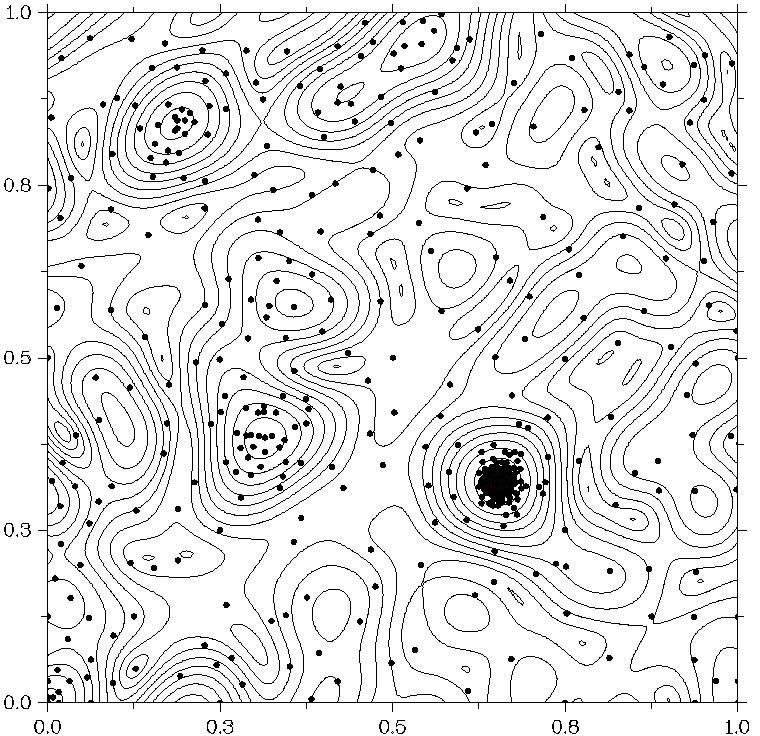
\includegraphics[width=0.75\textwidth]{fig1.jpg} 
  \caption{Problem solution $u(t)$} \label{fig11} 
\end{center}
\end{figure}

Thus, for a particle of a given mass $m>0$ it is necessary to determine its own frequency $\omega_0$, the amplitudes $A_i$, frequencies $\omega_i$ and phases $\varphi_i$ of the control action, as well as the initial conditions $u_0=u(0), \dot{u}_0=\dot{u}(0)$ for the equation (\ref{Eq:2}), such that conditions 1--3 are true.

Using the following notation for the equation (\ref{Eq:2}) solution 
\begin{equation}\label{Eq:3}
u(t,\omega,c)=\sum^{n}_{i=0}\left[c_{2i+1}\sin(\omega_it) + c_{2i+2}\cos(\omega_it)\right],	
\end{equation}
where  $c=\left(c_1,\ldots,c_{2n+2}\right)$, $\omega=\left(\omega_0,\omega_1,\ldots,\omega_n\right)$, we can represent the original problem as a constrained maximization problem with parameters  $c$ and $\omega$:
\begin{eqnarray} \label{Eq:4}
  & \left| \dot{u}(t_3,\omega,c) \right| \rightarrow \max \nonumber \\
  & \left|u(t_i,\omega,c)-q_i\right|\leq\delta, \; i=1,2,3, \\
	& \left|u(t,\omega,c)-q_0\right|\leq\delta, \; t\in[a,b]. \nonumber 
\end{eqnarray}

Solving the optimization problem (\ref{Eq:4}) and finding the vectors $\omega$, $c$ the solution to the original problem (\ref{Eq:2}) can be written in accordance with the following relationships: 
\begin{eqnarray} \label{Eq:5}
  & u_0=\sum^{n}_{i=0}c_{2i+2}, \; \; \dot{u}_0 = \sum^{n}_{i=0}c_{2i+1}\omega_i \nonumber \\
  & A_i=\left(\omega^2_0-\omega^2_i\right)\sqrt{c^2_{2i+1}+c^2_{2i+2}}\;, \; 1\leq i\leq n, \\
	& \varphi_i=\arcsin\frac{c_{2i+2}}{\sqrt{c^2_{2i+1}+c^2_{2i+2}}}\;, \; 1\leq i\leq n. \nonumber 
\end{eqnarray}

As follows from formula (\ref{Eq:3}), the parameters $c$ are included in the equation solution linearly, and the parameters $\omega$ -- non-linearly. Given the constraints (\ref{Eq:4}) this allows the problem to be reformulated and $c$ to be found without using a numerical optimization method.

Let's consider a set of points $(\tau_j,u_j), 0\leq j\leq m$, with the coordinates defined as follows:
\begin{eqnarray} \label{Eq:6}
  & \tau_j=a+jh, \; u_j=q_0, \; 0\leq j\leq m-3,\\
  & \tau_{m-2}=t_1, u_{m-2}=q_1, \nonumber \\
	& \tau_{m-1}=t_2, u_{m-1}=q_2, \nonumber \\
	& \tau_{m}=t_3, u_{m}=q_3, \nonumber
\end{eqnarray}
where $h=(b-a)/(m-3)$, i.e. the first $m-3$ points are located at equal distances in the center of the ''tube'', the other three align with the centers of the ''windows''.

The requirement is that the trajectory of particle $u(t)$ passes ''near'' the points  $(\tau_j,u_j), 0\leq j\leq m$. If the measure of deviation from the points is defined as the sum of the squared deviations
\[
\Delta(c,\omega)= \sum^{m}_{j=0}\left[u_j-u(\tau_j,\omega,c)\right]^2, 
\]
then the parameters $c$ can be found (given fixed values of $\omega$), by solving  the least squares problem
\begin{equation}\label{Eq:7}
c^\ast(\omega) = \arg \min\Delta(c,\omega).	
\end{equation}
According to the least squares method, the solution to problem (\ref{Eq:7}) can be obtained by solving a system of linear algebraic equations regarding the unknown $c$, which can be done, e.g., by Gaussian elimination.

It should also be considered that the components of frequency vector $\omega$ can be placed in ascending order, so as to avoid duplicate solutions corresponding to the vector $\omega$ with similar components in different order. In addition, it is natural to assume that frequencies in the control action must not just be ordered but differ by a certain positive value, as an actual physical device can only generate control signals with a certain precision. This assumption can be represented in the form of a requirement for the following inequalities to be true:
\begin{equation}\label{Eq:8}
\omega_{i-1}(1+\alpha)-\omega_i(1-\alpha)\leq 0, \; 1\leq i \leq n.	
\end{equation}
Here $\alpha\in(0,1)$ is a parameter reflecting the precision of signal generation by the control device.

Then the original problem can be reformulated as follows:
\begin{equation}\label{Eq:9}
\omega^\ast = \arg \max_{\omega \in \Omega} \left| \dot{u}(t_3,\omega,c^\ast(\omega)) \right|
\end{equation}
\[
\omega_{i-1}(1+\alpha)-\omega_i(1-\alpha)\leq 0, \; 1\leq i \leq n,
\]
\[
\left|u(t_i,\omega,c^\ast(\omega))-q_i\right|\leq\delta, \; i=1,2,3,
\]
\[
\max_{t\in[a,b]}{u(t,\omega,c^\ast(\omega))}-\min_{t\in[a,b]}{u(t,\omega,c^\ast(\omega))}\leq\delta,
\]
where $c^\ast(\omega)$ is determined from (\ref{Eq:7}), and the number of constraints will be dependent on the number of frequencies $n$ in the control action.

Fig.~\ref{fig11} shows trajectory $u(t)$, which corresponds to the solution to problem (\ref{Eq:9}) with parameters $a=1$, $b=10$, $t_1=13$, $t_2=16.65$, $t_3=18$, $q_0=q_3=0$, $q_1=7.65$, $q_2=-9.86$. The solution (with three significant digits)
\begin{eqnarray} \nonumber 
u(t)= \; &34.997\sin(0.01t-0.061)+11.323\sin(0.902t-0.777)- \nonumber \\
      &-19.489\sin(1.023t+0.054)+9.147 \sin(1.139t+0.633) \nonumber
\end{eqnarray}
is determined by the optimal vectors $\omega^\ast =(0.01, 0.902 , 1.023, 1.139)$ and $c^\ast=( 34.93, -2.151, -8.075, -7.936, 19.461, 1.048, -7.375, 5.411)$. As follows from (\ref{Eq:5}), the original problem with the solution $u(t)$ is noted as 
\begin{eqnarray} \nonumber 
\ddot{u}+10^{-4}u = & -9.213\sin(0.902t-0.777)-20.383\sin(1.023t+0.054)- \nonumber \\
                    &-11.842 \sin(1.139t+0.633), \nonumber \\
                    &u_0= -3.62, \; \dot{u}_0 = 4.556.\nonumber
\end{eqnarray}


\section{Generating a series of problems}\label{Sec:3}

The numeric experiments described below used a generator based on the approximation problem from Section \ref{Sec:2}. Apparently, the variation in any parameter of the original problem (\ref{Eq:2}) will change the optimization problem (\ref{Eq:9}), so it is sufficient to vary just a few of them.

The centers of the first two ''windows'', i.e. the pairs  $(t_1, q_1)$ and $(t_2, q_2)$, were chosen as the parameters for determining the specific problem statement. The values $q_1$ and $q_2$ were chosen independently and uniformly from the ranges  $[1,10]$ and $[-10, -1]$, respectively. The values $t_1$ and $t_2$ were dependent: first, the value $t_1$ was chosen from the range $[b+1, t_3-2]$, then, the value $t_2$ was chosen from the range $[t_1+1, t_3-1]$. All other parameters in problem (\ref{Eq:2}) were fixed: $a=1$, $b=10$, $t_3=18$, $q_0=q_3=0$, $\delta=0.3$. Parameter $\alpha$ from (\ref{Eq:8}) was chosen at $0.05$. The number of points in the additional grid $(\ref{Eq:6})$ for solving the least square problem (\ref{Eq:7}) was set at $20$. The problem of one-dimensional maximization and minimization from (\ref{Eq:9}) were solved by a scanning over a uniform grid of $100$ nodes within the interval $[a,b]$.

An important feature determining the existence of a feasible solution for the problem being considered is the number and range of frequency variation in the vector $\omega$. If the range is too small, or the number of frequencies is insufficient, the feasible domain in the problem (\ref{Eq:9}) will be empty. In the experiments carried out, the number of frequencies was chosen to be $n=3$, which corresponds to $\omega=(\omega_0,\omega_1,\omega_2,\omega_3)$, while the variable frequency change range was set from 0.01 to 2, i.e. $\omega_i\in[0.01, 2]$, $0\leq i\leq 3$.

Let's note some important properties of the problems produced by the generator under consideration.

\textbf{Remark 1}. Problem constraints (\ref{Eq:9}) are different in terms of the time required to verify them. For example, checking each of the first $n$ constraints in (\ref{Eq:9}) (let's call these constraints \textit{geometric})
\[
\omega_{i-1}(1+\alpha)-\omega_i(1-\alpha)\leq 0, \; 1\leq i \leq n,
\]
requires performing only three operations with real numbers. Testing other constraints (we will call them the \textit{main constraints}) 
\[
\left|u(t_i,\omega,c^\ast(\omega))-q_i\right|\leq\delta, \; i=1,2,3,
\]
\[
\max_{t\in[a,b]}{u(t,\omega,c^\ast(\omega))}-\min_{t\in[a,b]}{u(t,\omega,c^\ast(\omega))}\leq\delta
\]
is far more labor-intensive. First, this requires producing a system of linear equations to solve the problem (\ref{Eq:7}) ($\sim m(2n+2)^2$ computing of $\sin$ and $\cos$). Second, this system needs to be solved ($\sim \frac{2}{3}(2n+2)^3$ operations on real numbers). Third, two one-dimensional optimization problems need to be solved at the last constraint in (\ref{Eq:9}) ($\sim 100$ computing of $\sin$ and $\cos$).

\textbf{Remark 2}. The problems are characterized by multiextremal constraints, which form a non-convex feasible domain. For example, Fig.~\ref{fig:fig2} show level lines for the functions in the right-hand sides of the main constraints for one of the problems, while Fig.~\ref{fig:fig6} shows level lines of the objective function. These lines are provided within the feasible domain of the geometric constraints.
\begin{figure*}
	\centering
		\hfil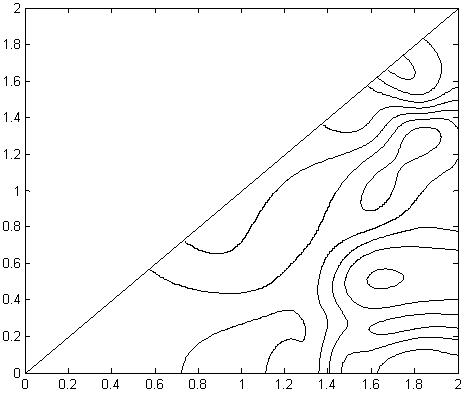
\includegraphics[width=0.49\textwidth]{fig2.JPG}
		\hfil %qquad
		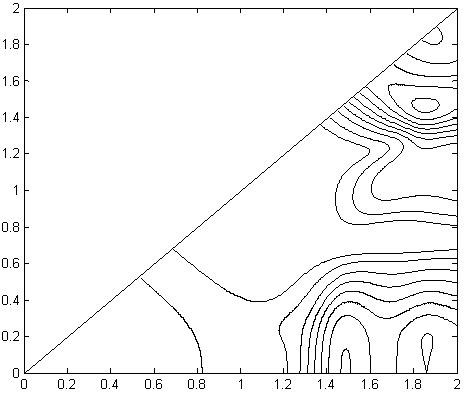
\includegraphics[width=0.490\textwidth]{fig3.JPG}
		\\[3ex] \hfil%qquad
		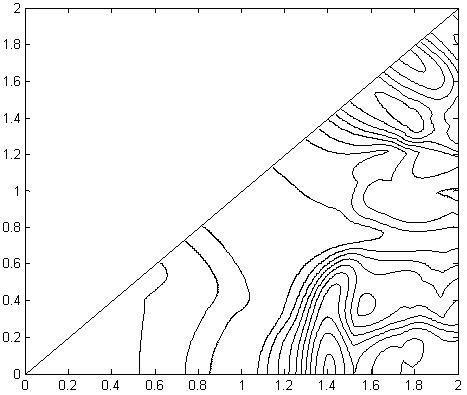
\includegraphics[width=0.490\textwidth]{fig4.JPG}
		\hfil %qquad
		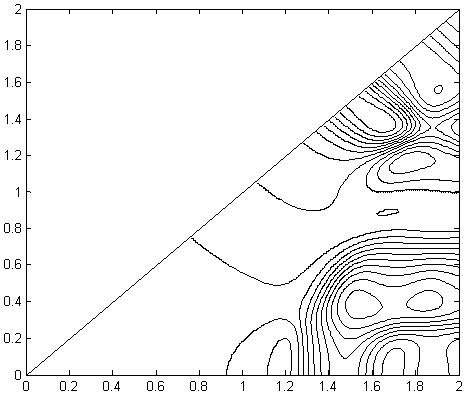
\includegraphics[width=0.490\textwidth]{fig5.JPG}
		\hfil
	\caption{Level lines for the main constraints} \label{fig:fig2}	
\end{figure*}
\begin{figure}
	\centering
		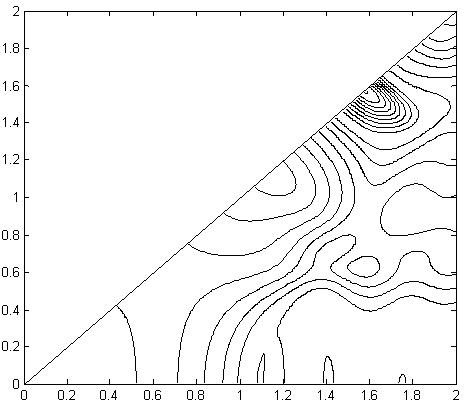
\includegraphics[width=0.50\textwidth]{fig6.JPG} 
	\caption{Level lines for the objective function} \label{fig:fig6}	
\end{figure}

\textbf{Remark 3}. Increasing the frequency change range results in new solutions appearing in an area of higher frequencies; the feasible domain of the optimization problem becomes multiply connected. For example, Fig. \ref{fig:fig7} shows two trajectories, the solid line corresponds to the vector $\omega =(0.01, 0.902, 1.023, 1.139)$ and solution
\begin{eqnarray*} 
u(t)= \; &34.997\sin(0.01t-0.061)+11.323\sin(0.902t-0.777)-  \\
      &-19.489\sin(1.023t+0.054)+9.147 \sin(1.139t+0.633) 
\end{eqnarray*}
obtained at  $\omega_i\in[0.01, 2]$, $0\leq i\leq3$, dashed line corresponds to the frequency vector  $\omega=(1.749, 1.946, 2.151, 2.377)$ and solution 
\begin{eqnarray*} 
u(t)= \; &5.434 \sin( 1.749 t + 0.832 ) + 12.958 \sin( 1.946 t + 0.241)+  \\
      &+11.844 \sin( 2.151 t - 1.377 ) + 4.302 \sin( 2.377 t + 0.501)
\end{eqnarray*}
obtained at $\omega_i\in[0.01, 4]$, $0\leq i\leq 3$. Obviously, the second solution is better, as the trajectory at the last point has the largest slope.

\begin{figure}
\begin{center}
  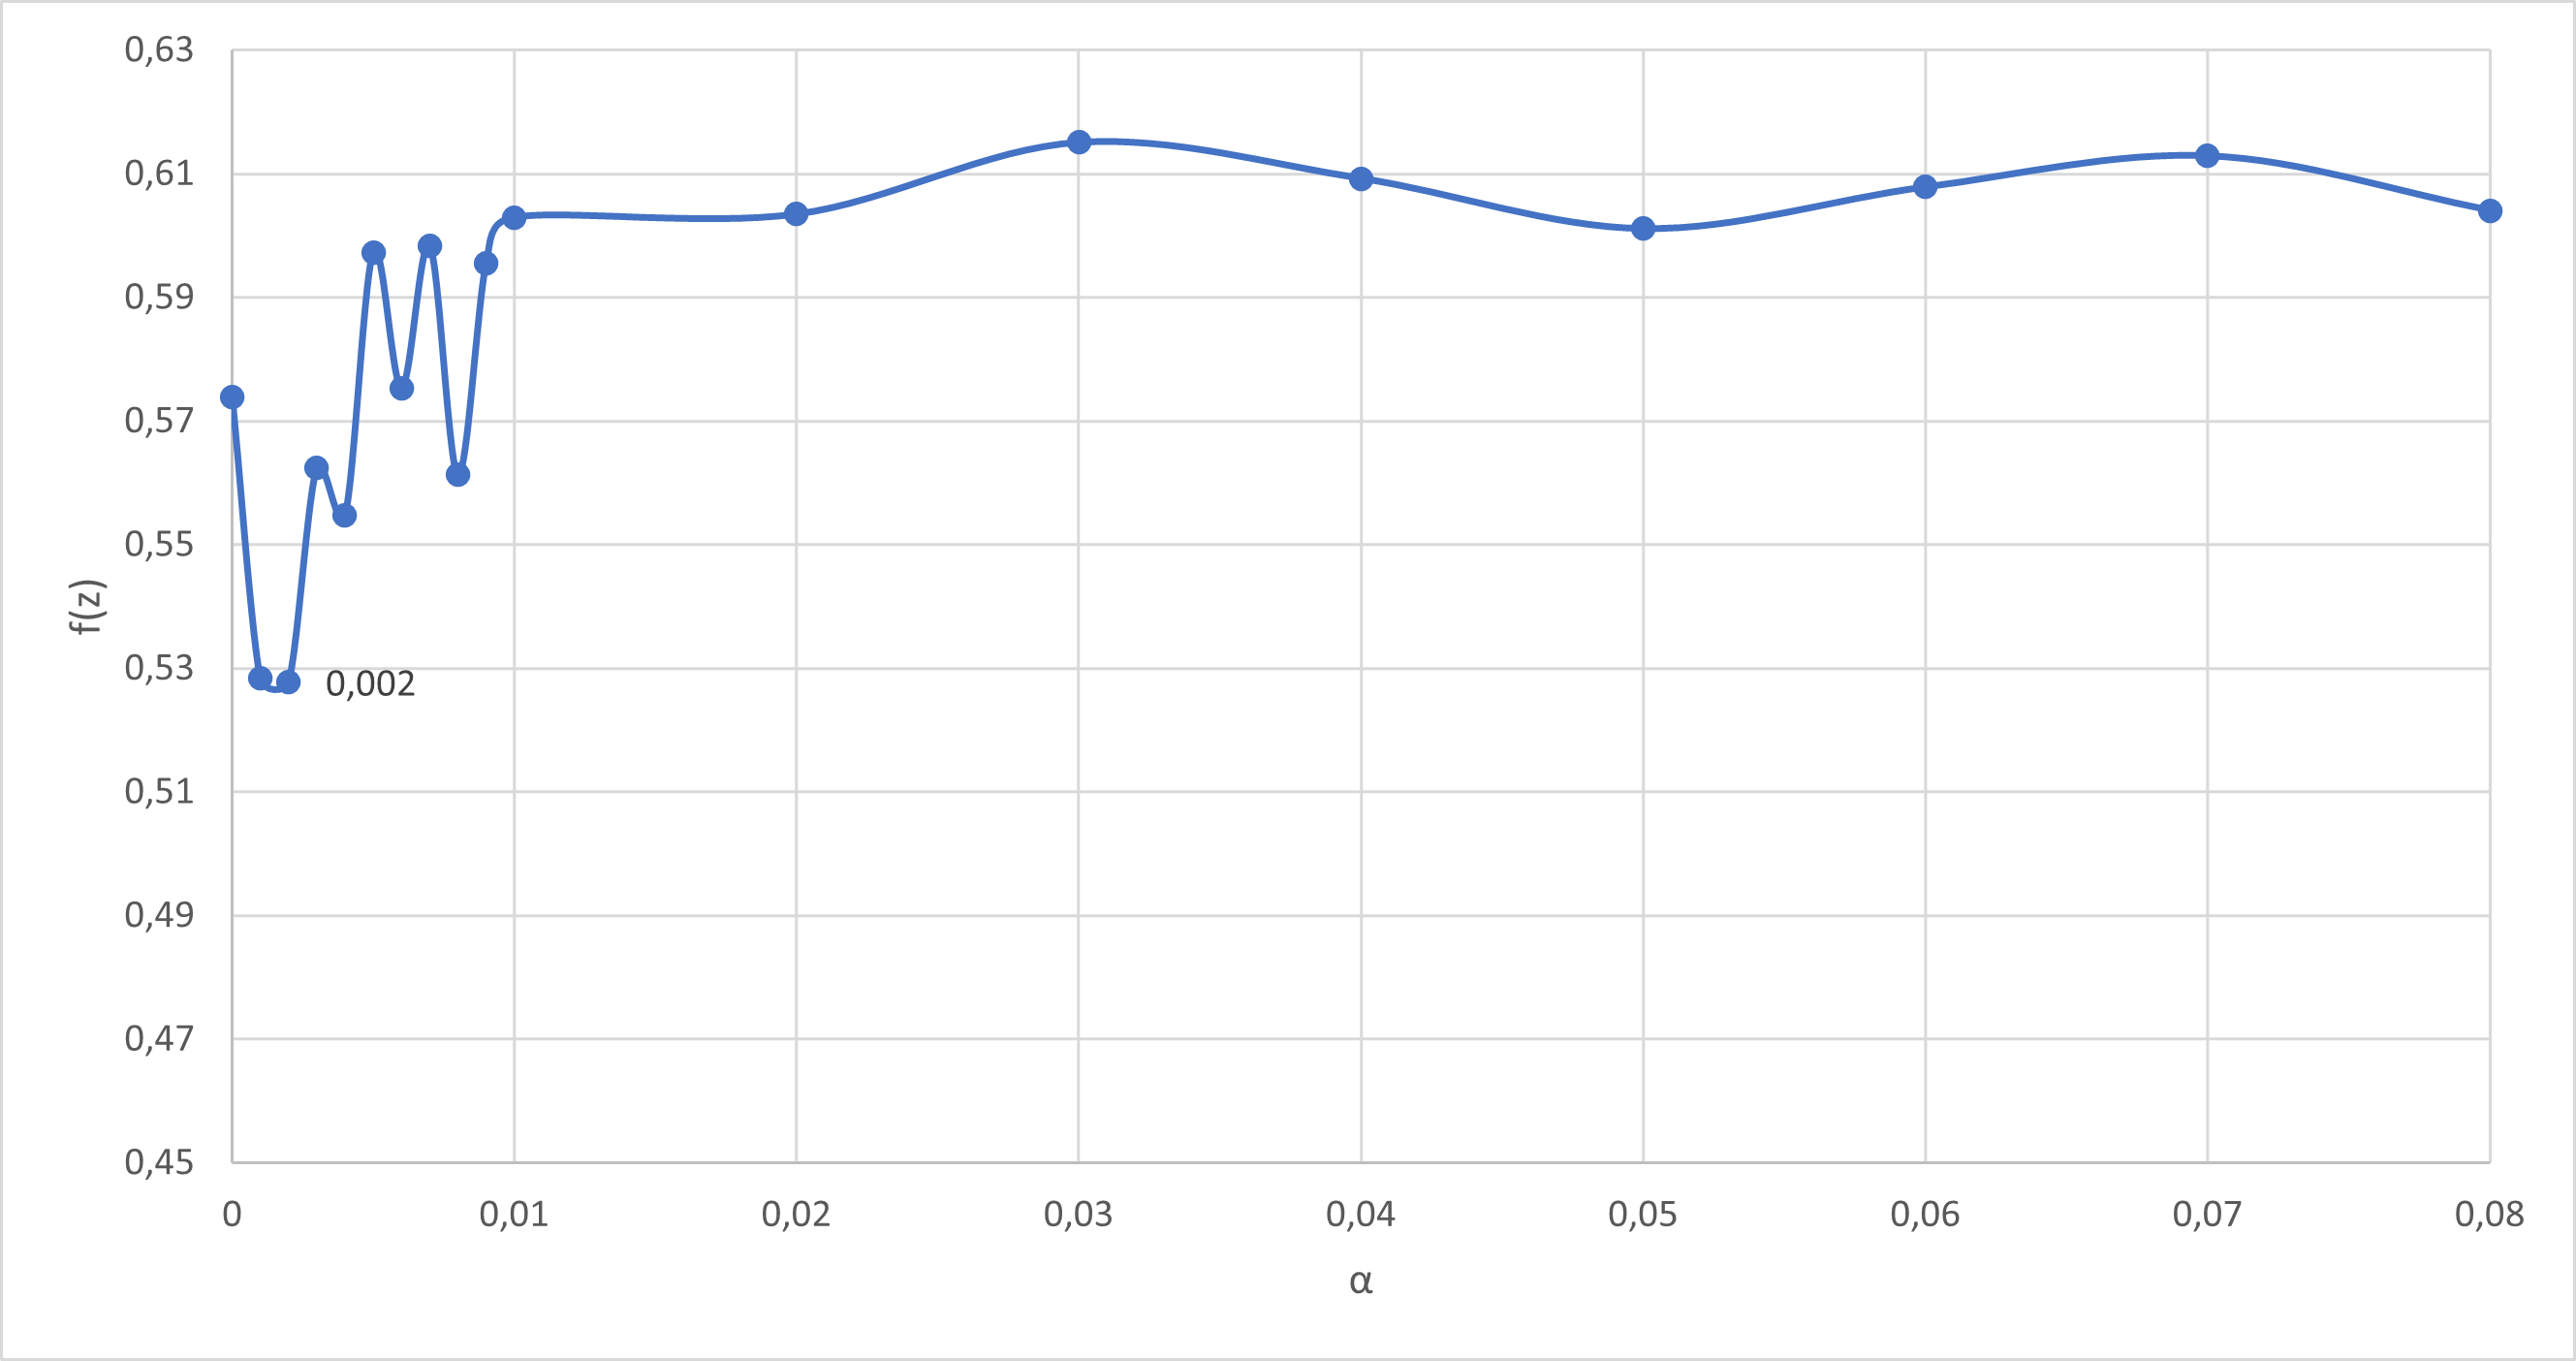
\includegraphics[width=0.75\textwidth]{fig7.jpg} 
  \caption{Solutions with different frequencies}\label{fig:fig7} 
\end{center}
\end{figure}

These optimization problem properties allow us to conclude that this generator may be applied for testing parallel global optimization algorithms. 
%new text
%Ознакомиться с обзором подходов к распараллеливанию оптимизационных алгоритмов итересующиеся читатели могут в книге [Pardalos1992]. В рамках данного исследования мы будем применять параллельные алгоритмы, основанные на информационно-статистическом подходе [Strongin2000, 2013].
Interested readers may find the review of approaches to parallelization of optimization algorithms in \cite{Pardalos1992}. In this study we will use a parallel algorithm based on information-statistical approach \cite{Strongin2000,Sergeyev2013}.

\section{Parallel global optimization index algorithm}

Let's consider a multiextremal optimization problem in the form
\begin{equation}\label{Eq:11}
\varphi(y^\ast)=\min{\left\{\varphi(y): y\in D, g_j(y)\leq 0, 1\leq j\leq m\right\}},
\end{equation}
where the search domain $D$ is represented by a hyperparallelepiped
\begin{equation}\label{Eq:12}
D={\left\{y\in R^N: a_i\leq y_i\leq b_i, 1\leq i\leq N\right\}}.
\end{equation}
Suppose, that the objective function $\varphi(y)$ (henceforth denoted by $g_{m+1}(y)$) and the left-hand sides $g_j(y), \; 1\leq j \leq m,$ of the constraints satisfy Lipschitz condition 
\[
\left|g_j(x_1)-g_j(x_2)\right|\leq L_j\left\|y_1-y_2\right\|, 1\leq j \leq m+1, y_1,y_2\in D.
\]
with respective constants $L_j, \; 1 \leq j \leq m+1,$ and may be multiextremal.
Then, it is suggested that even a single computing of a problem function value may be a time-consuming operation since it is related to the necessity of numerical modeling in the applied problems (see, for example, \cite{Grishagin2015,Modorskii}).


Using a continuous single-valued mapping$y(x)$ (Peano-type space-filling curve) of the interval  $[0,1]$ onto $D$ from (\ref{Eq:12}), a multidimensional problem (\ref{Eq:11}) can be reduced to a one-dimensional problem
\begin{equation}\label{Eq:13}
\varphi(y(x^\ast))=\min{\left\{\varphi(y(x)): x\in [0,1], \; g_j(y(x))\leq 0, \; 1\leq j\leq m\right\}},
\end{equation}
The reduction of dimensionality matches the multidimensional problem with a Lipschitzian objective function and Lipschitzian constraints with a one-dimensional problem where the respective functions satisfy the uniform H{\"o}lder condition (see \cite{Strongin2000}), i.e. 
\[
\left|g_j(y(x_1))-g_j(y(x_2))\right|\leq K_j\left|x_1-x_2\right|^{1/N}, \;\;\; x_1,x_2\in [0,1], \;\; 1\leq j\leq m+1.
\]
Here $N$ is the dimensionality of the original multidimensional problem, and the coefficients $K_j$ are related to Lipschitz constants $L_j$ with formulae 
\[
K_j\leq 2L_j \sqrt{N+3}, \; 1\leq j\leq m+1.
\]
The issues around the numeric construction of a Peano-type curve and the corresponding theory are considered in detail in \cite{Strongin2000,Sergeyev2013}. Here we can just state that the numerically computed curve (\textit{evolvent}) is an approximation of the theoretical Peano curve with a precision at least $2^{-m}$ for each coordinate (the parameter \textit{m} is called the \textit{evolvent density}).

Let's introduce the classification of points $x$ from the search domain $[0,1]$ using the \textit{index}  $\nu=\nu(x)$. This index $\nu$ is determined by the following conditions:
\[
g_j(y(x))\leq 0, \;\;1 \leq j\leq \nu -1,\;\; g_\nu(y(x))>0,
\]
where the last inequality is negligible if $\nu=m+1$, and meets the inequalities $1\leq \nu=\nu (x) \leq m+1$. This classification produces a function
\[
f(y(x))=g_\nu (y(x)), \; \nu=\nu(x),
\]
which is determined and computed along the interval $[0,1]$. Its value in a point $x$ is either the value of the left part of the constraint violated at this point (in the case, when $\nu \leq m$), or the value of the objective function (in the case, when $\nu = m+1$). Therefore, determining the value $f(y(x))$ is reduced to a sequential computation of the values
\[
g_j(y(x)), \; 1 \leq j \leq \nu=\nu(x),
\]
i.e. the subsequent value $g_{j+1}(y(x))$ is only computed if $g_j(y(x)) \leq 0$. The computation process is completed either when the inequality $g_j(y(x))>0$ becomes true, or when the value of $\nu(x)=m+1$ is reached.

The procedure called \textit{trial} at point  $x$  automatically results in determining the index $\nu$ for this point. The pair of values  
\begin{equation}\label{Eq:16}
z=g_\nu(y(x)), \; \nu = \nu (x),
\end{equation}
produced by the trial in point $x \in [0,1]$, is called the \textit{trial result}.

A serial index algorithm for solving one-dimensional conditional optimization problems (\ref{Eq:13}) is described in detail in \cite{Barkalov2002}. This algorithm belongs to a class of characteristical algorithms (see \cite{Grishagin1997}). It can be parallelized using the approach described in \cite{Grishagin1997} for solving unconstrained global optimization problems. Let's briefly describe the rules of the resulting \textit{parallel index algorithm} (PIA).

Suppose we have $p \geq 1$  computational elements (e.g., CPU cores), which can be used to run $p$ trials simultaneously. In the first iteration of the method, $p$ trials are run in parallel at various random points $x^i\in(0,1)$, $1\leq i \leq p$. 
Suppose $n \geq 1$  iterations of the method have been completed, and as a result of which, trials were carried out in $k=k(n)$ points $x^i, 1\leq i \leq k$. Then the points $x^{k+1},...,x^{k+p}$  of the search trials in the next $(n+1)$-th iteration will be determined according to the rules below.

\begin{enumerate}
\item 
Renumber the points $x^1,...,x^k$ from previous iterations with lower indices, lowest to highest coordinate values, i.e.
\begin{equation}\label{Eq:17}
0=x_0<x_1<...<x_i<...<x_k<x_{k+1}=1,
\end{equation}
and match them with the values $z_i=g_\nu(y(x_i))$, $\nu=\nu(x_i)$, $1 \leq i \leq k$, from (\ref{Eq:16}) , calculated at these points; points $x_0=0$ и $x_{k+1}=1$ are introduced additionally; the values $z_0$ и $z_{k+1}$ are indeterminate.
\item
Classify the numbers $i,1\leq i \leq k$, of the trial points from (\ref{Eq:17}) by the number of problem constraints fulfilled at these points, by building the sets
\begin{equation}\label{Eq:18}
I_\nu = \left\{i: 1 \leq i \leq k,\ \nu = \nu(x_i)\right\},\ 1 \leq \nu \leq m+1,
\end{equation}
containing the numbers of all points $x_i,1\leq i \leq k$, with the same values of $\nu$. The end points $x_0=0$ and $x_{k+1}=1$ are interpreted as those with zero indices, and they are matched to an additional set $I_0={0,k+1}$. 

Identify the maximum current value of the index
\begin{equation}\label{Eq:19}
M=\max \left\{\nu = \nu(x_i), \ 1\leq i \leq k\right\}.
\end{equation}
\item
For all values of $\nu, \ 1\leq \nu \leq m+1$, calculate the values  
\begin{equation}\label{Eq:20}
\mu_\nu = \max \left\{ \frac{\left|z_i-z_j\right|}{\left(x_i-x_j\right)^{1/N}} : i,j \in I_\nu, j<i\right\}.
\end{equation}
If the set $I_\nu$ contains less than two elements or $\mu_\nu$ from (\ref{Eq:20}) equals zero, then assume $\mu_\nu=1$.
\item
For all non-empty sets $I_\nu$, $1 \leq \nu \leq m+1$, determine the values
\begin{equation}\label{Eq:21}
  z^\ast_\nu =  
   \begin{cases}
    -\epsilon_\nu,  \nu < M, \\
    \min{\left\{g_\nu(x_i):i\in I_\nu\right\}}, \nu = M,
   \end{cases}
\end{equation}
where $M$ is the maximum current value of the index, and the vector
\begin{equation}\label{Eq:22}
\epsilon _R=\left(\epsilon_1,...,\epsilon_m\right),
\end{equation}
with positive coordinates is called the \textit{reserve vector} and is used as a parameter in the algorithm.
\item
For each interval $(x_{i-1},x_i)$,$1 \leq i \leq k+1$, calculate the \textit{characteristic} $R(i)$: 
\[
R(i)=\Delta_i+ \frac{(z_i-z_{i-1})^2}{(r_\nu\mu_\nu)^2\Delta_i}-2\frac{z_i+z_{i-1}-2z^\ast_\nu}{r_\nu\mu_\nu},\;\; \nu=\nu(x_{i-1})=\nu(x_i),
\]
\[
R(i)= 2\Delta_i-4\frac{z_i-z^\ast_\nu}{r_\nu\mu_\nu},\;\; \nu(x_{i-1})<\nu(x_i)=\nu,
\]
\[
R(i)= 2\Delta_i-4\frac{z_{i-1}-z^\ast_\nu}{r_\nu\mu_\nu},\;\; \nu = \nu(x_{i-1})>\nu(x_i).
\]
where $\Delta_i=(x_i-x_{i-1})^{1/N}$, and the values $r_\nu>1, 1\leq\nu\leq m+1$, are used as parameters in the algorithm.
\item
Reorder the characteristics $R(i)$, $1\leq i \leq k+1$, from highest to lowest 	
\begin{equation}\label{Eq:23}
R(t_1)\geq R(t_2)\geq ... \geq R(t_{k})\geq R(t_{k+1})
\end{equation}
and choose $p$ largest characteristics with interval numbers $t_j, 1\leq j \leq p$.
\item
Carry out $p$ new trials in parallel at the points $x^{k+j}, 1 \leq j \leq p$, calculated by the formulae
\begin{eqnarray*}
& x^{k+j}=\frac{x_{t_j}+x_{t_j-1}}{2}, \; \nu(x_{t_j-1})\neq \nu(x_{t_j}), \\
& x^{k+j}=\frac{x_{t_j}+x_{t_j-1}}{2}- \frac{\mathrm{sign}(z_{t_j}-z_{t_j-1})}{2r_\nu}\left[\frac{\left|z_{t_j}-z_{t_j-1}\right|}{\mu_\nu}\right]^N, \; \nu(x_{t_j-1})=\nu(x_{t_j})=\nu. \\
\end{eqnarray*} 

%Добавить результаты испытаний в информационную базу алгоритма, и перейти к правилу 1.
\end{enumerate}

The algorithm stops if the condition $\Delta_{t_j}\leq \epsilon$ becomes true for at least one number $t_j, 1\leq j \leq p$; here  $\epsilon>0$ has an order of magnitude of the desired coordinate accuracy.

Let's formulate the conditions for algorithm convergence. For this, in addition to the exact solution $y^\ast$ of the problem (\ref{Eq:11}), we will also consider the \textit{$\epsilon$-reserved solution}, determined by the conditions
\[
\varphi(y_\epsilon)=\min{\left\{\varphi(y): y\in D, \; g_j(y)\leq -\epsilon _j, \; 1\leq j\leq m\right\}},
\]
where $\epsilon_1,...,\epsilon_m$ are positive numbers  (''reserves'' for each constraint). Let's also introduce the set
\begin{equation}\label{Eq:27}
Y_\epsilon=\left\{y\in D: g_j(y)\leq 0, \; \varphi(y)\leq\varphi(y_\epsilon)\right\}
\end{equation}
of all feasible points for the problem (\ref{Eq:11}), which are no worse (in terms of the objective function's value) than  $\epsilon$-reserved solution.

Using this notation, the convergence conditions can be formulated as the theorem below.

\textbf{Theorem}. Suppose the following conditions are true:
\begin{enumerate}
\item
The problem  (\ref{Eq:11}) has $\epsilon$-reserved solution $y_\epsilon$.
\item
Each function  $g_j(y)$, $1\leq j \leq m+1$, satisfies Lipschitz condition with the respective constant $L_j$.
\item
The parameters  $\epsilon_j, \; 1 \leq j \leq m,$ from  (\ref{Eq:22}) have the values of the respective coordinates from the reserve vector $\epsilon_R$.
\item
For the values  $\mu_\nu$ from (\ref{Eq:20}) starting from a certain iteration, the following inequalities are true:
\[
r_\nu\mu_\nu>2^{3-1/N}L_\nu\sqrt{N+3}, \ 1 \leq \nu \leq m+1.
\]
\item
Each iteration uses a fixed number of computational elements  $p$, $1<p<\infty$, and each trial is completed by a single computational element within a finite time.
\end{enumerate}

Then any accumulation point $\bar{y}$ of the sequence $\left\{y^k\right\}$ generated by parallel index method while solving the problem (\ref{Eq:11}) is admissible and satisfies the conditions 
\[
\varphi(\bar{y})=\inf \left\{\varphi(y^k):g_j(y^k) \leq 0, 1 \leq j \leq m, k=1,2,...\right\}\leq \varphi (y_\epsilon).
\]
i.e., $\bar{y}$ belongs to the set $Y_\epsilon$ from (\ref{Eq:27}).

These convergence conditions proceed from the theorem of convergence of the serial index algorithm \cite{Strongin2000} and the theorem of convergence of a synchronous characteristical algorithm  \cite{Grishagin1997}.

\section{Results of numerical experiments}

%new text
The procedure applied to evaluate the efficiency of the algorithm uses an \textit{operating characteristics} method, originally  described in \cite{Grishagin1978}, which consists of the following.

Suppose a problem from the series under consideration be solved by a certain algorithm. The problem is associated with the sequence of trial points $\left\{y(x^k)\right\}$ produced by the algorithm. The sequence is truncated either when a trial point falls (for the first time) into a certain $\epsilon$-vicinity of the solution $y^*$ or when a certain number of trials $K$ does not produce such a point. In our experiments we used $K=10^6$.

The results obtained by solving all problems in a series by means of the algorithm is represented by the function $P(k)$ defined as the fraction of problems in which some trial point fall within the given  $\epsilon$-neighborhood of the solution in the first $k$ steps. This function is called the \textit{operating characteristic} of the algorithm.

Since the specification of an $\epsilon$-vicinity requires that $y^*$ be known, its value was estimated in advance (for each problem) by searching through all nodes of a uniform grid (defined on the search domain), e.g. with a step $10^{-2}$ by coordinates.

As discussed above (see Remark 1 from Section \ref{Sec:3}), the constraints in the problem being addressed have a different nature. The first three constraints are geometric, and checking whether they are feasible is not hard. Checking other constraints is far more labor-intensive. Therefore, when building operating characteristics for this class of problems, we will only consider the trials that resulted in checking labor-intensive constraints. The trials that were completed while checking geometric constraints are not included in the total number of trials.

The experiments were carried out for the parallel index algorithm (PIA) described above, with the number of used cores $p$ varying from 1 to 8. The parameters used were $r_\nu=2.5, 1\leq\nu\leq 8$. Components of the reserve vector from (\ref{Eq:22})  were selected adaptively under the rule $\epsilon_\nu=0.005\mu_\nu, 1\leq\nu\leq 7,$ where $\mu_\nu$ is from (\ref{Eq:20}) (see \cite{Strongin2000} for a justification of this component selection for the reserve vector). Computing experiments were carried out on one of the nodes of a high-performance cluster of the Nizhny Novgorod State University. The cluster node includes Intel Sandy Bridge E5-2660 2.2 GHz CPU and 64 Gb RAM. For implementation of the parallel algorithm OpenMP was used.

The algorithm's operating characteristics when using different number of computing cores $p$ obtained with a series of $100$ problems, are shown in Fig.~\ref{fig:fig8}. The location of the curves shows that any of the parallel algorithms solve 100\% of the problems in less than $7 \cdot 10^5$ trials, with more than 80\% of the problems completing within $2 \cdot 10^5$  trials. The operating characteristics also show that the algorithm is \textit{non-redundant} -- the number of trials in the parallel algorithm does not grow (compared to serial algorithm) when additional cores are employed. 
\begin{figure}[h]
\begin{center}
  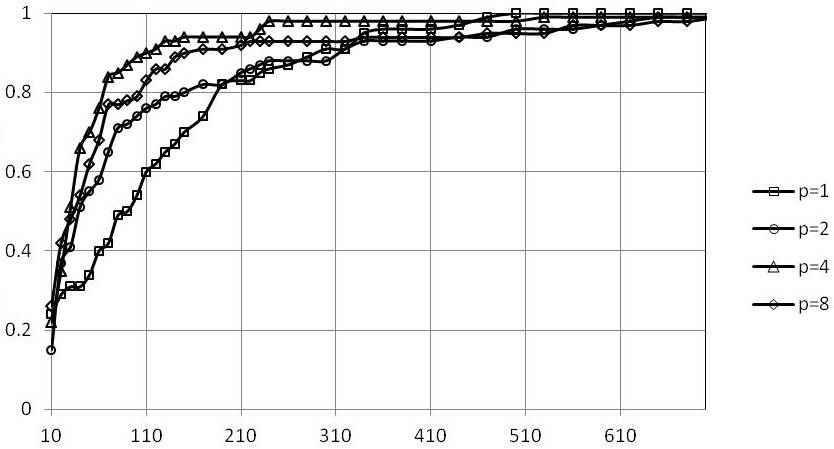
\includegraphics[width=0.9\textwidth]{fig8.jpg} 
  \caption{Operating characteristics of PIA, which uses $p$ cores }\label{fig:fig8} 
\end{center}
\end{figure}

Now let's evaluate the speedup achieved by using a parallel index algorithm, depending on the number $p$ of computing cores used. Table~\ref{tab:comparison} shows the average number of iterations $n(p)$ performed by the algorithm when solving a series of $100$ problems, and speedup by the iterations $s(p)$ of a parallel algorithm. 
\begin{table}
	\caption{Speedup of the algorithm}
	\label{tab:comparison}
	\center
	\begin{tabular}{ccc}
		\hline\noalign{\smallskip}
	   $p$ & $n(p)$ & $s(p)$  \\
	  \noalign{\smallskip} \hline \noalign{\smallskip}		
	   1 &	241239 &	-- \\
		 2 &	94064 &	2.56 \\
		 4 &	45805 &	5.27 \\
		 8 &	22628 &	10.66 \\
		\noalign{\smallskip}\hline
	\end{tabular}
\end{table}
The results show that the speedup is greater than the number of cores used (hyper-acceleration). This situation is explained by the fact that the algorithm performs an adaptive evaluation of the behavior of the objective function (calculating the lower bounds for the Lipschitz constant (\ref{Eq:20}) and the current minimum value (\ref{Eq:21})). For example, if the Lipschitz constant is better estimated in a parallel version, then the parallel algorithm using $p$ cores can be accelerated by more than $p$ times. 

\section {Conclusion}

In summary, we must note that the method proposed in this work to generate multidimensional conditional global optimization problems allows:

\begin{itemize}
	\item clear visualization of the best current estimate and the final solution to the problem, regardless of the number of variables;
	\item increased dimensionality of the optimization problem being addressed by varying the original approximation problem;
	\item control of the feasible domain by adding extra non-convex constraints.
\end{itemize}
The functions included in the optimization problem are computationally intensive, which also differentiates the mechanism proposed from other known mechanisms.

The proposed generator was used to build and subsequently solve 100 problems using a parallel index algorithm. The operating characteristics of the parallel algorithm have been built, clearly demonstrating its non-redundancy.

\bigskip \textbf{Acknowledgments.} This study was supported by the Russian Science Foundation, project No 16-11-10150.

\begin{thebibliography}{99}

\bibitem{Hill}
Hill, J.D.: A search technique for multimodal surfaces. IEEE Transactions on Systems Science and Cybernetics. 5(1), 2--8 (1969)

\bibitem{Toropov}
Toropov, V.V.: Simulation approach to structural optimization. Structural Optimization. 1, 37 -- 46 (1989)

\bibitem{Shekel}
Shekel J.: Test functions for multimodal search technique. Proceedings of the 5th Princeton Conference on Information Science Systems. Princeton, Princeton University Press. 354--359 (1971)

\bibitem{Globalizer}
Strongin, R.G., Gergel, V.P., and Tropichev, A.V.: Globalizer. Investigation of minimizing sequences generated by global search algorithms for univariate functions. User's guide. Nizhny Novgorod University Press., Nizhny Novgorod (1995)

\bibitem{Strongin2000}
Strongin, R.G., Sergeyev, Ya.D.: Global optimization with non-convex constraints. Sequential and parallel algorithms. Kluwer Academic Publishers, Dordrecht (2000)

\bibitem{Barkalov2002}
Barkalov, K.A., Strongin, R.G.: A global optimization technique with an adaptive order of checking for constraints. Computational Mathematics and Mathematical Physics 42(9), 1289--1300 (2002)

\bibitem{Grishagin1997}
Grishagin, V.A., Sergeyev, Ya.D., Strongin, R.G.: Parallel characteristical algorithms for solving problems of global optimization. J. Glob. Optim. 10(2), 185--206 (1997)

\bibitem{Gergel1999}
Sergeyev, Y.D., Grishagin, V.A.: Sequential and parallel algorithms for global optimization. Optimization Methods and Software. 3, 111--124 (1994)
%Gergel, V.P., Sergeyev, Ya.D.: Sequential and parallel algorithms for global minimizing functions with Lipschitzian derivatives. Computers and Mathematics with Applications, 37(4-5), 163--179 (1999)

\bibitem{Grishagin2001}
Sergeyev Ya.D, Grishagin V.A.: Parallel asynchronous global search and the nested optimization scheme. Journal of Computational Analysis and Applications. 3(2), 123--145 (2001)

\bibitem{Grishagin2016} 
Gergel, V., Grishagin, V., Gergel, A.: Adaptive nested optimization scheme for multidimensional global search. J. Glob. Optim. 66(1), 35--51 (2016)

\bibitem{Gaviano}
Gaviano, M., Kvasov, D.E, Lera, D., and Sergeyev, Ya.D.: Software for generation of classes of test functions with known local and global minima for global optimization. ACM Transactions on Mathematical Software 29(4), 469--480 (2003)

\bibitem{Kvasov2006} 
Sergeyev, Ya.D., Kvasov D.E.: Global search based on efficient diagonal partitions and a set of Lipschitz constants. SIAM J. Optim. 16(3), 910--937 (2006)

\bibitem{Sergeyev2010} Lera D., Sergeyev Ya.D. Lipschitz and Holder global optimization using space-filling curves, Applied Numerical Mathematics, 60(1-2), 115--129 (2010)

\bibitem{Paulavicius2014} 
Paulavicius, R., Sergeyev, Y., Kvasov, D., Zilinskas, J.: Globally-biased DISIMPL algorithm for expensive global optimization. J. Glob. Optim. 59(2-3), 545--567 (2014)

\bibitem{SergeyevKvasov2015} 
Sergeyev, Y.D., Kvasov, D.E.: A deterministic global optimization using smooth diagonal auxiliary functions. Communications in Nonlinear Science and Numerical Simulation. 21(1-3), 99--111 (2015)

\bibitem{Pardalos1990}
Floudas, C.A., Pardalos, P.M.: A collection of test problems for constrained global optimization algorithms. LNCS. 455 (1990)

\bibitem{Floudas1999}
Floudas, C.A., et al.: Handbook of test problems in local and global optimization.  Springer (1999)

\bibitem{Pardalos1992}
Pardalos, P.M., Phillips, A.T., Rosen, J.B.: Topics in parallel computing in mathematical programming. Science Press, New York (1992)

\bibitem{Sergeyev2013} 
Sergeyev, Ya.D., Strongin, R.G., Lera, D.: Introduction to global optimization exploiting space-filling curves. Springer (2013)

\bibitem{Grishagin2015}
Gergel, V.P., Kuzmin, M.I., Solovyov, N.A., Grishagin, V.A.: Recognition of surface defects of cold-rolling sheets based on method of localities. International Review of Automatic Control 8(1), 51--55 (2015)

\bibitem{Modorskii}
Modorskii, V.Y., Gaynutdinova, D.F., Gergel, V.P., Barkalov, K.A.: Optimization in design of scientific products for purposes of cavitation problems. In: Simos T.E. (Ed.) ICNAAM 2015, AIP Conference Proceedings. 1738, art. no. 400013 (2016)

\bibitem{Grishagin1978}
Grishagin, V.A.: Operating characteristics of some global search algorithms. Problems of Stochastic Search. 7, 198--206 (1978) [in Russian]
                                                                           
\end{thebibliography}

\end{document}